%% Example document for the eis_msc_thesis document class. Compile with
%% pdfLaTeX or LaTeX.
%%
%% Created: April 7, 2004, by Johan Carlson
%% Last modified: June 7, 2009, by Johan Carlson


%% Pick one of the following depending on the language of the report, and if 
%% you want twosided or onesided print.
%% Also change language definition after \begin{document}

% English, twosided
\documentclass[12pt,a4paper,openright,final,twoside,en]{csee_msc_thesis} 

% English, onesided    
%\documentclass[12pt,a4paper,openright,final,oneside,en]{csee_msc_thesis}     

% Swedish, twosided
%\documentclass[12pt,a4paper,openright,final,twoside,sv]{csee_msc_thesis}     

% Swedish, onesided
%\documentclass[12pt,a4paper,openright,final,oneside,sv]{csee_msc_thesis}     

%%==================================================================
%% Class options specific to this class
%%==================================================================
%%   en, sv  - Swedish or English
%%   parskip - Use blank row instead of indentation for
%%             new paragraphs
%%==================================================================

%% These packages are not required in general,
%% only for some examples in this document.
\usepackage{fancybox}
\usepackage{verbatim}
\usepackage{url}

\begin{document}

%%==================================================================
%% Define variables here
%%==================================================================

\def\thesistitle{Bachelor Thesis\\
                Use of DANE to improve the security for identity federations}
\def\theauthor{Sophia Bergendahl, Christoffer Holmstedt}
\def\theaddress{Lule� University of Technology\\
            Dept.\ of Computer Science and Electrical Engineering}

% Define the English abstract
\def\theabstract{Identity federations is a way to build a standard for online services similar to the one in real life with identification cards and signatures.
However, there are more security aspects to take in to account online.
This report analysis the security mechanism used to achieve data integrity in an identity federation and specifically the use of X.509 certificates as well as an evaluation of the possibility to use DNS-Based Authentication of Named Entities (DANE) to improve the security for an identity federation.
Moreover, the report describes different protocols, standards and some about the underlying technology that is used in identity federations and DANE. 
The report is a result of literature studies, set up of test environment and discussions with experts.
It concludes that improvements can be made on how identity federations handle their own metadata and trust other entities metadata. 
DANE is today only a draft, but when DANE with TLS/TLSA becomes a RFC and when a standard for how DANE handles SAML certificates
or certificates in general is specified, it can be used to improve the initial trust bonding.

%and its documents needs to more restricted and the metadata sharing within SAML is the achilles heel.
%that DANE can be used for improvements
%need trust in identity federations
%therefore increasing security is important
%this is what this is about, how to use DANE with identity federations.

%ABSTRACT \- what the report is about and puts it in a global perspective.

%Abstract to be written TODO

%This is an example document of how to use the
%\texttt{csee\_msc\_thesis} document class.

%The document class supports both Swedish and English theses, double
%or single sided print.
}
\def\thepreface{It's an interesting world we live in where we are constantly on the move with our cellphones, laptops and other devices online day out and day in, all hours during the day.
With the increase of possibilities online we are eager to find a way to build trust online for even more feature rich online services.%, both in the private and public sector.

This thesis work was carried out at .SE (The Internet Infrastructure Foundation) in Sweden, at their Stockholm office in the spring of 2012, from the end of March to the beginning of June.
The subject for this thesis was chosen because of our interest in internet security.
Sophia's focus has been on identity federations and certificates while Christoffer has put more focus on DNS-Based Authentication of Named-Entites (DANE).

We would like to thank Staffan Hagnell (.SE) for giving us the opportunity to come and work for .SE and for the support on the way to our conclusions.
We would also like to thank Carl Ljungqvist (Certezza AB) for the first introduction about indentity federations and Rickard Bellgrim (Certezza AB) for giving us much needed help when setting up the testing environment as well as helping us understand how certificates are used in general and within identity federations.
For giving us new perspectives about DANE we would like to thank Jakob Schlyter (Kirei) and Leif Johansson (SUNET). 

From our university, Lule\r{a} University of Technology, we would like to thank our 
supervisor Ulf Bodin, Dept. of Computer Science, Electrical and Space Engineering, 
for guiding us in the right direction when struggling with the thesis and putting words to our conclusions.
We would also like to thank Johan Carlson, Dept. of Computer Science, Electrical and Space Engineering, 
for the LaTeX template that we have used for this report. 

As a final note we would like to thank all of you that has supported us in our work but didn't get mentioned above.
Thank you.




% It's an interesting world we live in where we are constantly on the move with our cellphones, laptops and other devices online day out and day in, all hours during the day.
% with the increase of possibilities online we are eager to find a way to build trust 
% online for even more feature rich online services directed to you specifically as a citizen, both in the private and public sector.
%
% With the advant of DNSSEC shaping up in production around the world new possiblities arises.

% PREFACE Explains when, where, and why the work was carried out and you can also
% acknowledge the people who have supported and helped you during the course of your
% work.

% The preface is the place where you can discuss some personal
% experiences with the project. This is also the place where you can
% thank people who helped you out.

\vspace*{1.5cm}%
\hfill Sophia Bergendahl and Christoffer Holmstedt
}
\def\thedate{\today}
%\def\thedate{Template version: \theclassversion , \theclassdate}

% Use this if you want a Swedish abstract
\def\theswedishabstract{\input{SweAbstract/sweabstract.tex}}

%%==================================================================
%% Generate preamble pages here (This should not need any changes)
%%==================================================================
\startpreamble
  {\thesistitle}
  {\theauthor}
  {\theaddress}
  {\theabstract}
  {\thepreface}
  {\thedate}
  {}
%  {\theswedishabstract} % use this for Swedish abstract, leave empty for English

%%==================================================================
%% Start including the chapters
%%==================================================================
% First argument is the "running titles", second is the chapter name.
\makechapter{Introduction}{Introduction\label{ch1}}
\section{Background}
In todays society more and more information is shared through internet.
A lot of the communication consist of sharing pictures, stories and information with friends and family.
The online websites that allow and promote these services are often very easy to use and especially easy to register a new account for.
To log in to most of these services the required credentials are often username and password. 
%which is deemed as a low assurance level \cite[p.~244]{pdf:SOU}.
%This has its pros and cons, though in the end, the above mentioned services might not need higher assurance level.

Services that require somekind of proof that the user behind the keyboard really is the person he/she says he/she is, are lagging behind in the online era.
A solution to this problem is "BankID" which was introduced in 2003 \cite{website:bankid-about} in Sweden.
Other solutions comes from Nordea, SEB, Telia, Posten and Steria \cite[p.~256]{pdf:SOU}.
All listed solutions have their pros and cons and a new solution is in the horizon.
A new solution will be built upon the concept of identity federations \cite[p.~23]{pdf:SOU}.

One major identity federation that exists in Sweden today is SWAMID, it's for students in higher education and is run by SUNET.
Another one is "Skolfederation.se" which is planned to go into production during 2013.
"Skolfederation.se" is for pupils/parents and teachers in compulsary primary and secondary school run by .SE and SUNET. 
Other federations that soon will come in to production is "E-legitimationsn{\"a}mden" \cite{website:elegnamnd} and "V\r{a}rd, h{\"a}lsa, omsorg" according to .SE.  

An identity federation does not have the goal to increase security and therefore will probably continue to use username and password. 
However, the federation provides user friendliness since the user only has to have one username and one password to all services within the federation. 

%As of today two major identity federations exists in Sweden.
%Those are SWAMID for students in higher education run by SUNET and "Skolfederation.se" for pupils/parents and teachers in compulsary primary and secondary school run by .SE and SUNET. "Skolfederation.se" is planned to go into production during 2013.


%In our thesis we dig deeper into the identity federation and examine how DNS-Based Authentication of Named Entities (DANE) 
%\cite{rfc:6394,rfc:draft-dane,rfc:draft-smime} can be used to improve the security in identity federations.

\section{Problem description}
The subject of the thesis is divided into smaller subsection. 
\\\\
- An analysis of the security mechanism used to achieve data integrity in an identity federation and specifically the use of X.509 certificates.
\\\\
- Two separate evaluations one about the possibility to use DANE to improve the security for an identity federation
and another one concern the possibility to implement support for DANE in the open source software package Shibboleth.
\\\\
- Implementation of DANE in Shibboleth, simpleSAMLphp or equivalent software to improve the security for an identity federation.

%Firstly, an analysis of the security mechanism used to achieve data integrity in an identity federation and 
%specifically the use of X.509 certificates.
%Secondly, two separate evaluations one about the possibility to use DANE to improve the security for an identity federation
%and another one concern the possibility to implement support for DANE in the open source software package Shibboleth.
%Finally, the implementation of DANE in Shibboleth, simpleSAMLphp or equivalent software to improve
%the security for an identity federation.

\section{Purpose}
The purpose with this thesis is to show that DNS-Based Authentication of Named Entities (DANE) \cite{rfc:6394,rfc:draft-dane,rfc:draft-smime} can be used to improve security for identity federations.
In the same time proving DNS Security Extension (DNSSEC) \cite{rfc:4033,rfc:4034,rfc:4035,rfc:5011} useful, since DANE is 
depending on the use of DNSSEC.

\section{Project delimitations}
As stated above this project will be about DANE and identity federations and as with most, if not all implementation of different protocols and standards, a lot of underlying technology is used.
This is also the case with DANE and identity federations.

Within an identity federation there are four main entities which are clients, service providers, identity providers and in most cases a federation operator.
All entities might communicate with each other over different protocols and communication schemes.
In this project the main focus has been on SAML2 over HTTPS.

A firm delimitation in this report is that of excluding how TLS/SSL works in detail and why it's deemed as a secure way for transmission between two hosts.
Some parts in the report will touch the topic of the TLS/SSL handshaking process but will not go into further detail.
The focus in this report is on the actual data that is being transmitted (SAML2 requests and responses) and how it's deemed secure. 

Another delimitation is made concerning DANE, DNS and DNSSEC.
DANE uses DNSSEC and DNS as an underlying technology and security schemes/protocols.
As the focus is on DANE, issues that might exist with DNS and DNSSEC in general is not discussed in this report.


%The other main part in this report is the one concerning DANE, DNS and DNSSEC.
%DANE uses DNSSEC and DNS as an underlying technology and security schemes/protocols.
%As the focus is on DANE, issues that might exist with DNS and DNSSEC in general is not discussed in this report.

%---
%INTRODUCTION 

%Background: A short background, the reason why the work was carried out, and why you chose that particular topic.

%Problem description: Problem area A broader discussion of what you are going to write about (the task). This can often be included under the same heading as the introduction. Formulating the problem leads to the purpose.

%Purpose: The purpose may for example be specified in a list of to clauses.

%Project delimitation: Arguments and boundaries. You must naturally give the reasons for your delimitations.


\makechapter{Method}{Method\label{ch2}}
\section{Approach}
%To be able to show that DANE can be used to improve the security in identity federation, more knowledge was needed in the specific subjects of concern.

To be able to answer the questions stated in "Problem area", more knowledge was needed in the specific subjects of concern.

The beginning of the project consisted mainly of a literature study about DANE, identity federations and the SAML 2.0 standard, which the federation that .SE is involved in is based on. 
Several discussions took place with experts in the different subjects to get other perspectives than those recieved from the literature study.

A test environment was set up to develop a deeper understanding about identity federations and SAML, as well as the software 
Shibboleth that was used. 
It was with recommendations by Staffan Hagnell the software choice to use Shibboleth was made, instead of simpleSAMLphp or equivalent software.
The test environment also included OpenLDAP as user credential storage, Bind as DNS server and OpenDNSSEC to be able to sign all DNS resource records.

With an improved understanding and knowledge, an analysis was possible and conclusions from the analysis could be used 
to start the implementaion phase. During the entire project a few hours per week were dedicated for writing this report.

%  Before -----------------------------


%The approach was to first read up about identity federations as well as talk to experts. 
%The identity federations in this report are based on the SAML 2.0 standard which is the standard used for both SWAMID and skolfederation.se.
 
%To understand identity federations, SAML and Shibboleth better, a test environment using Shibboleth was put online at "danetest.se". 
%In the test environment one service provider and one identity provider was used to keep it as simple as possible while still being able to see and log all data flows.
%It was by recommendations the software choice to use Shibboleth was made, instead of simpleSAMLphp or equivalent software.
%The test environment also included OpenLDAP as user credential storage, Bind as DNS server and OpenDNSSEC to be able to sign all DNS resource records.

%When basic understanding of the identity federation and SAML had been achieved DANE was up next.
%As with identity federation most information is available in standard documents such as RFCs and drafts.

%An analysis of all aquired information took place before transitioning in to the implementation phase.
%During the entire project a few hours per week were dedicated for writing this report.


%--------------------------------------------------------------------------------------------------------------

% More about the service- and identity provider and other entities in the identity federation is described in the thesis. 

% After reading up on identity federations, we read up about DANE, through drafts, by following the DANE mailing list and by talking to experts. DANE demands that DNSSEC is used and therefore some reading was also done about DNSSEC. We also read up more about TLS/SSL to easier understand where DANE is needed in the identity federation.

%When the analysis was finished, we had found possible places where DANE could be used and we could start implementing.

%\section{Investigation description}

%\section{Discussion of alternative methods}

%\section{Reliability and validity}


%METHOD in longer theses, it is appropriate for the author to define; 
% his or her approach.
% All reports must contain a sufficiently detailed description of; 
% how the investigation was carried out as to allow it to be repeated by someone else and 
% a discussion of alternative methods(strengths and weaknesses). 
% The concepts; 
% reliability and validity have a given place when issues of method are dealt with.






\makechapter{Theory}{Theory\label{ch3}}
\section{Identity federations}
\subsection{What is an identity federation?}
A simple identity federation example is when signing in to "antagning.se". 
The user visits "antagning.se", needs to visit "my pages", to do so he/she presses "Log in". 
Assuming the user is already studying in Sweden perhaps at Lule\r{a} University of Technology he/she 
can select this university among the listed universities. 
The user has made his/her choice and is redirected to the selected university's student portal and is identified through the university.
When the user is verified he/she is redirected back to "antagning.se" with an approval message.

An identity federation can be based on different standards.
The identity federation used in the thesis work testing environment is based on OASIS Security Assertion Markup Language (SAML 2.0) \cite{pdf:oasis-open-core,pdf:oasis-open-metadata,pdf:oasis-open-metadata-profile,pdf:oasis-open-bindings,pdf:oasis-open-profiles,pdf:oasis-open-glossary,pdf:oasis-open}. 
The SAML technical overview \cite[p.~8]{pdf:oasis-open} describes SAML as an XML-based framework both for
describing and exchanging security information between business partners online.    

\begin{figure}[ht]
\begin{center}
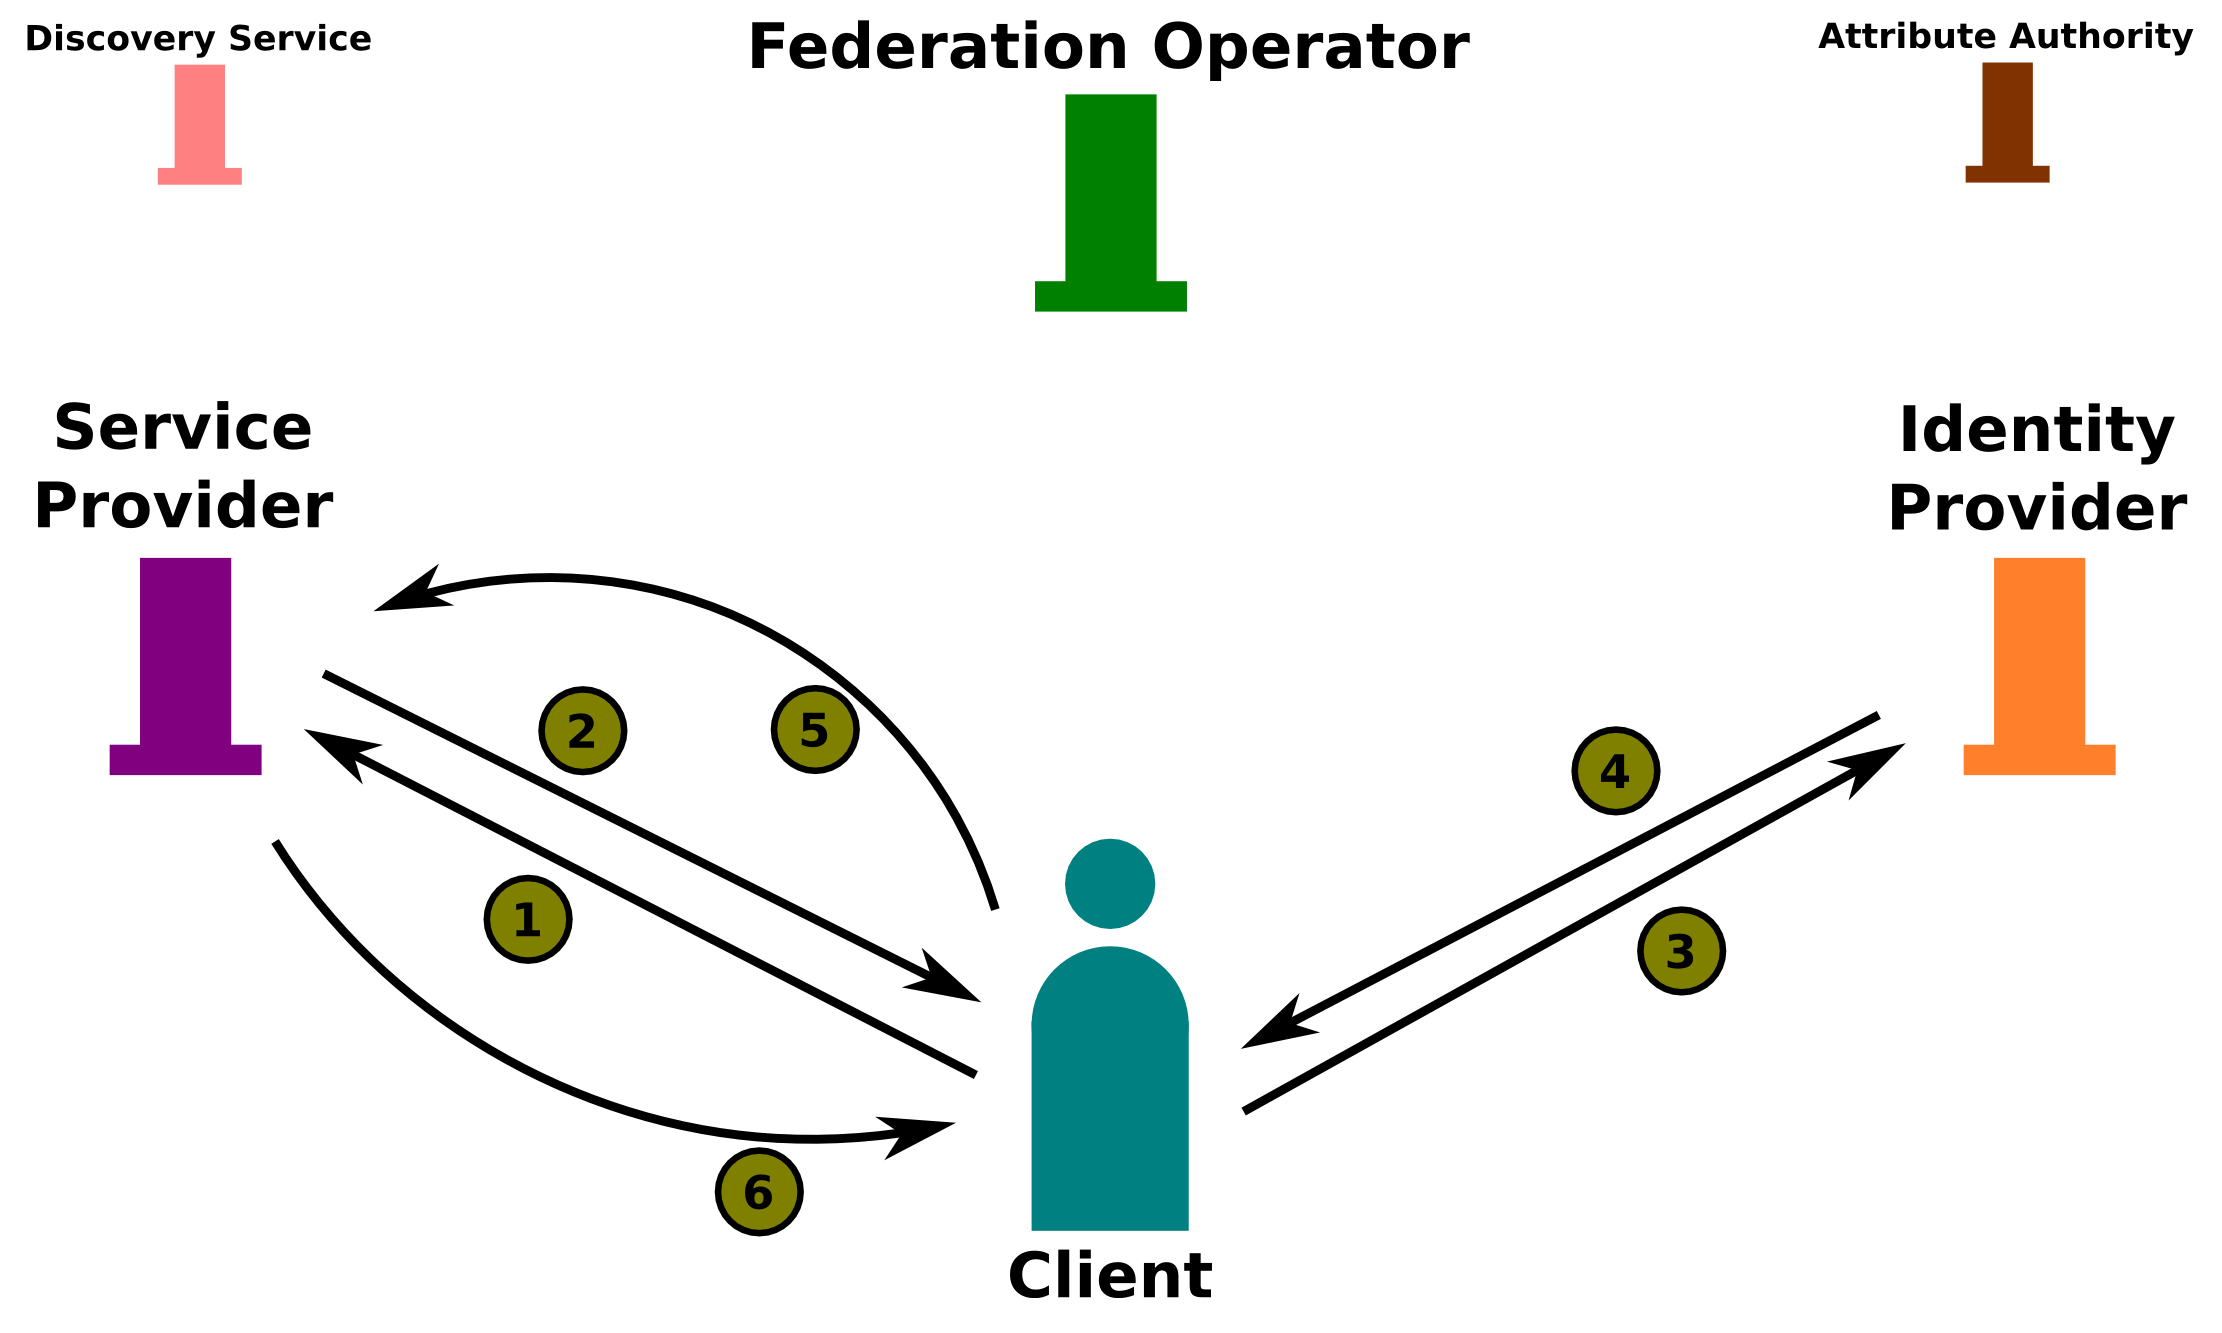
\includegraphics[scale=1]{Figures/identityFed.png}
\end{center}
\caption{Shows how the client visits the service provider (1). 
The client want to see restricted resources at the service provider, whom demands that the client is identified first. 
Therefore, the service provider redirects the client to the identity provider (2) and (3). 
At the identity provider, the client is authenticated and sent back to the service provider (4) and (5). 
The client is now allowed to see restricted resources at the service provider (6).\label{ch3:IdentityFed}}
\end{figure}

In SAML standard "antagning.se" is a Service Provider (SP) \cite[p.~11]{pdf:oasis-open-glossary} and the identification at 
Lule\r{a} University of Technology is the Identity Provider (IdP) \cite[p.~7]{pdf:oasis-open-glossary}, see figure \ref{ch3:IdentityFed}.
The Discovery Service (Disco) is where the user could chose from several universities at "antagning.se".
Furthermore, SAML also specifies the Attribute Authority (AA) that provides 
a "ticket" containing information about the user from a third party perspective.
A theoretical AA example is "Bolagsverket" (Swedish Companies Registration Office).
"Skatteverket" (Swedish Tax Agency) wants to allow individuals to see their business' tax account and sends an attribute request to "Bolagsverket" that will answer this request with a "ticket" containing information that allows or disallows the individual to see his/her tax account \cite[p.~284]{pdf:SOU}.

Outside of the SAML standard, the identity federation can also have a Federation Operator (FO). It is possible to have an identity federation both with and without a federation operator. 
The federation operator provides digitally signed aggregated metadata \cite[p.~3]{pdf:Skolfederation}. 
The SAML Technical Overview \cite[p.~16]{pdf:oasis-open} says "Metadata defines a way to express and share configuration information between SAML parties.
For instance, an entity's supported SAML bindings, operational roles (IDP, SP, etc), identifier information,
supporting identity attributes, and key information for encryption and signing can be expressed using SAML
metadata XML documents. SAML Metadata is defined by its own XML schema".
The key information refers to the shared certificates (public keys) that are used when connecting and sending requests and responses 
messages between the entities.
With that said every service provider and identity provider holds the shared certificates between each other within its metadata. 

The need of a federation operator grows as the amount of service- and identity providers increase,
since it is easier to turn to the federation operator to make sure the metadata is up to date 
instead of having to turn to each other. 
The only thing is that the service- and identity providers has to keep track of a shared certificate with the federation operator, 
meanwhile, the federation operator provides them with a metadata file containing all certificates within the federation.
A federation operator also provides a unity between the entities in the federation. This unity can be used so that every entity share 
administration, has the same technical set up and so on.

\subsection{The technical side of an identity federation}
The example with "antagning.se" is in SAML referred to as a SP-initiated web SSO  \cite[p.~12]{pdf:oasis-open}, 
where SSO stands for Single Sign-On and SP for Service Provider. SSO is when it is possible to sign in at one place and use that identification at other places as well. 

SP-initiated web SSO uses The Web Browser SSO Profile \cite[p.~14]{pdf:oasis-open-profiles} that says that "to implement this scenario,
a profile of the SAML Authentication Request protocol is used, in conjunction with the HTTP Redirect, HTTP POST and
HTTP Artifact bindings".

In more technical terms the SP-initiated web SSO scenario is in the SAML Profiles document \cite[p.~15]{pdf:oasis-open-profiles} described as the client (principal) sends an HTTP request via an HTTP user agent asking to access a protected resource at the service provider.
The client is not authenticated and therefore the service provider obtains with the authentication request protocol the location to the identity provider. The service provider then issues an "AuthnRequest" message that the user agent deliver to the identity provider through an HTTP redirect, post or artifact binding.
At the identity provider the client is identified through some back-end engine with user credentials.
The identity provider then issues a "Response" message that the user agent deliver to the service provider through HTTP post or artifact binding.
This message holds at least one authentication assertion as well as attributes that describes the user or it may hold an error.
Depending on the response message the client will receive access to the service provider or not.
\section{Certificates}
\subsection{X.509 certificates}

This section describes how certificates are used to send a private message from Alice to Bob, the technical steps from encryption 
of the message to the validation of trust.
The example is based on the introduction on SSL/TLS from the Apache Foundation \cite{website:ssl_intro}.
%Alice and Bob with the help of a signed certificates and is based on\cite{website:ssl_intro}. 

Public key cryptography algorithm transforms a message from Alice in to a private (encrypted) message to Bob, 
the message is unreadable until it is decrypted. 
Encrypted messages can only be decrypted with a secret key, in public key cryptography two keys are used that both can encrypt and 
decrypt messages. 
However, if one key is used to encrypt the message only the other key can decrypt it, which make publication of the public key 
possible while keeping the private key secret. 
Additionally, if Alice and Bob has shared keys, Alice can encrypt the private message with the public key and only Bob 
with the private key can decrypt the message.

The possibility that someone has made changes to the message still exist since the public key is public. 
"Message digest" even called one-way function or hash function can be used to guarantee that the message has not changed. 
Message digest creates a short, fixed-length representation of the message about to be sent and sends the message and
the summary to Bob.
Then, when Bob receives the message he makes a summary as well and compares it with Alice's.

In addition, the message digest has to be securely sent as well, which is made possible with digital signatures. A digital signature
is made by the private key by encrypting a digest of the message and other information as well, sequence number for example.
It is Alice that creates the digital signature and includes it in the message digest to Bob and since no one can change the digest and still 
sign it, the integrity is kept. Moreover, to make sure reuse of the signature can not be made at a later date, the signature contains a 
sequence number that is unique. 

Furthermore, Alice needs to know that the shared public key is with Bob as well as Bob needs to verify that the message signature 
really was signed by Alice's private key. With a certificate that validates the other's identity, confirms the public key and
is signed by a Certificate Authority (CA), Alice can be sure she is talking to Bob and vice versa.

\subsubsection{Certificates and security}
Certificates are not secure in themselves the security is built on cryptographic algorithms and most often on public-key cryptography as in the example above.
%\emph{"Cryptanalysis is about analysing and breaking ciphers"} \cite[p.~252]{book:computer-security}.
%It provides secure communication between the message sender and receiver. 
Cryptographic algorithms, which is a part of cryptanalysis, uses keys to protect data, in public-key cryptography a public encryption key and a private (secret) decryption key is used. \cite[p.~252]{book:computer-security}

The RSA algorithm has become almost synonymous with public key cryptography according to Computer Networking, A top down approach \cite[p.~726]{book:computer-networking}.
This book also informs that RSA uses arithmetic modulo-n operations as well as it describes how the recipient generates his/her private and public RSA key.
RSA is secure since there are no known algorithms that quickly can factor large prime numbers and the larger the generated prime numbers are, the more secure the keys become.

\subsection{Certificates in SAML}

Saml2int \cite{website:saml2int} describes an Interoperable SAML V2.0 Web Browser SSO Deployment Profile that is based on 
SAML Web Browser SSO Profile in the SAML Profiles document \cite{pdf:oasis-open-profiles}. 
The deployment profile describes the behaviour and options that all parties are supposed to follow. 
Furthermore, it addresses the content, exchange and processing of SAML messages.
For example in the Saml2int profile \cite{website:saml2int}, the service provider should at endpoint protect response 
messages using Transport Secure Layer (TLS) or Secure Sockets Layer (SSL)  and identity providers should do the same when receiving 
authentication request. 
However, if an identity provider does not use TLS/SSL, XML Encryption should be used and in its response message return an encrypted assertion. 
In addition, if service providers does not use TLS/SSL as recommended, then the service providers metadata should include a suitable key descriptor for XML Encryption.

%A TLS/SSL handshake example adapted to the identity federation influenced by \cite{website:ssl_explained}.
%The client initiates the handshake by connecting to the service provider with TLS/SSL on port 443. 
%Continues with sending basic information to the service provider, whom respond with sending basic 
%information as well as its certificate and public key back. 
%The client validates the certificate and public key with the CA as mentioned in certificates in general above. 
%Additionally, if the validation was successful the client generates a secret key to be used during the session and 
%sends the key encrypted to the service provider completing the handshake. 

\section{DNS-Based Authentication of Named Entities} 
\subsection{In general}
DANE, DNS-based Authentication of Named Entities, is as of writing still a new concept and technology.
It's introduced with the informational RFC6394 document \cite{rfc:6394} describing some use cases and some parts specified in more detail in the Internet-Draft \emph{"The DNS-Based Authentication of Named Entities (DANE) Protocol for Transport Layer Security (TLS)"} \cite{rfc:draft-dane}.
After the specification for TLS communication, S/MIME is up next, which will describe how to map an emailaddress to a resource record.
Exactly how this will work and which resource record type that must be used is not yet clear according the to the draft \cite{rfc:draft-smime}.
Make note that these Internet-Drafts from the Internet Engineering Task Force (IETF) is still "work in progress" as they are still drafts and may change.

The problem that DANE tries to solve is the current issue with Certificate Authorities (CAs) where anyone of them may give out a certificate for any domain name.
It might not be likely that a CA loses its private key but might sign a certificate with information that is not correct or the CA might sign a key that is intended for signing/encrypting emails but is then used in other settings.
%It might not be likely that a CA signs a certificate that doesn't come from the true owner of a domain name though the CA might be hacked and lose their private key or the CA might sign a key that should be used for signing emails but is then used for something else.

%A hacker that gets hold of the private key of a CA would get the ability to create a new signed certificate for any domain of his/her choice.
A hacker that gets hold of a perfectly valid certificate from a well-known CA for a domain he/she doesn't own will be able to lure unexpected visitor to a fake site with TLS/SSL active.
As the model with CAs works today where they can sign any domain name and the more common webbrowsers (Mozilla Firefox, Microsoft Internet Explorer, Google Chrome) trust most of these CAs, the certificate from the hacker will give clients connecting to the server with the false certificate a "false-positive".
The domain name matches the common name in the certificate and it's signed by one of all trusted/well-known CAs.
This is where DANE comes in as a solution.

\begin{figure}[ht]
\begin{center}
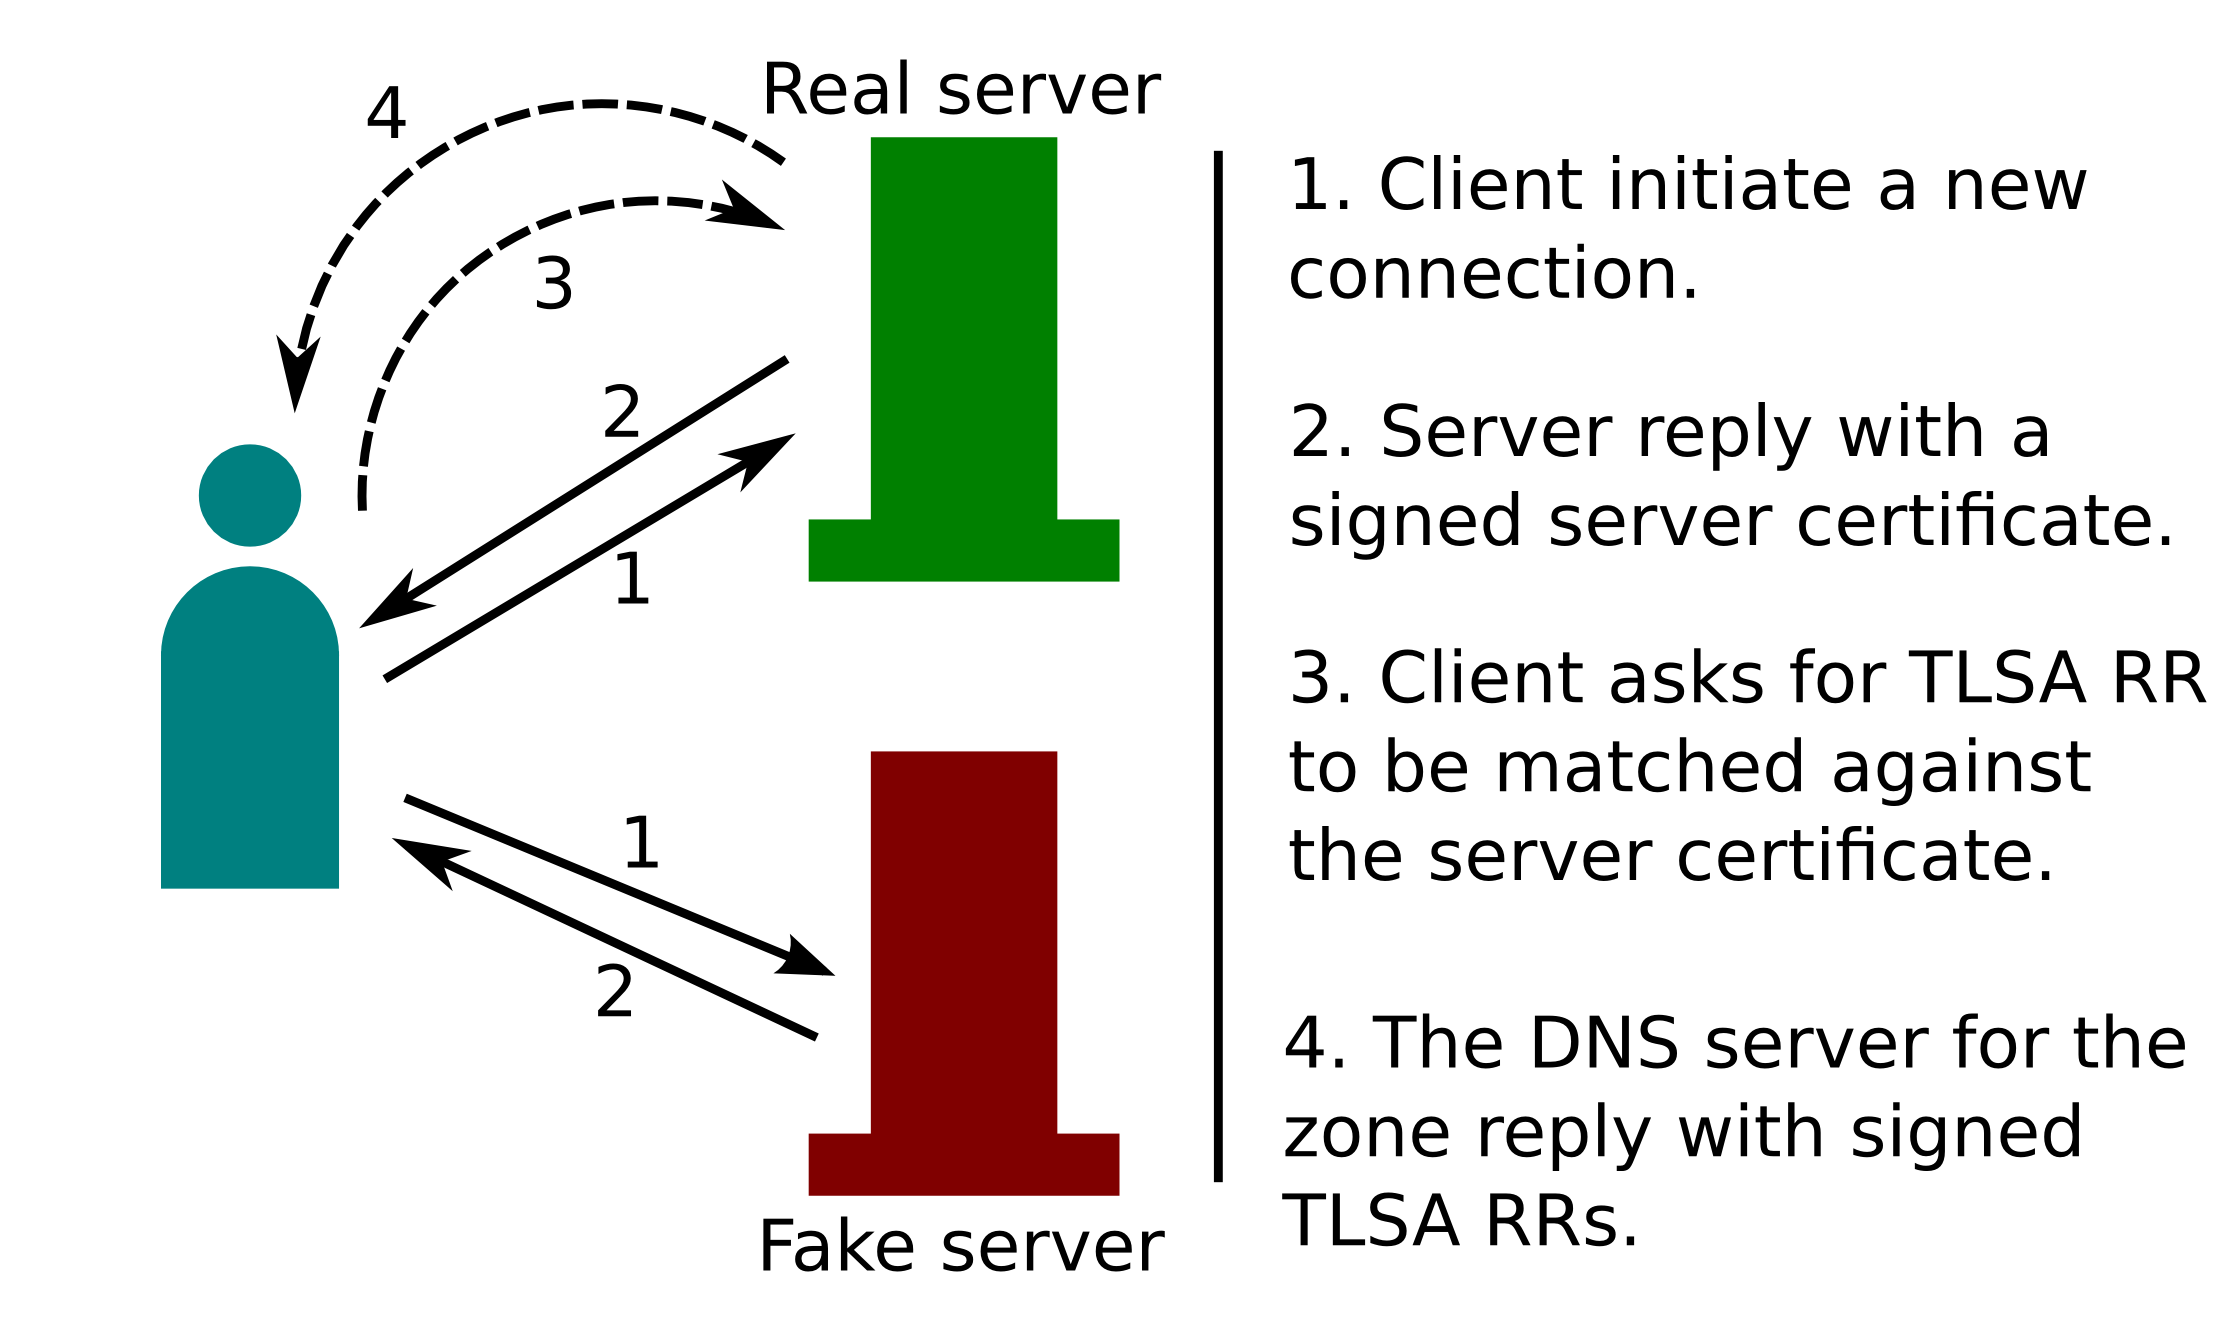
\includegraphics[scale=1]{Figures/daneWithTlsa.png}
\end{center}
\caption{A client connect to either a real or fake server. The third and fourth step is done within the Domain Name System and requires DNSSEC active. (It is assumed that both the real and the fake server has a server certificate signed by some well-known CA for the same domain.)\label{ch3:daneWithTlsa}}
\end{figure}

The following explanation is also presented in figure \ref{ch3:daneWithTlsa}.
If the client connecting to the false server could get some information about which certificate is the true one to use, the client would know that the false certificate is a false one and not to trust it.
In short, this works by trusting the DNSSEC infrastructure and the owner of a domain name can publish a TLSA DNS resource record (for TLS communication) which tells the client which certificate is the correct one to use.
If the hacker tried the same attack with DANE fully operational he/she would not succeed cause the client would know that the false certificate from the hacker (fake server) is actually a false one.
%This is what happens in figure \ref{ch3:daneWithTlsa} when the client can compare the server certificate (recieved in step 2) with the TLSA resource record (recieved in step 4).
The client would in this case immidiately drop all established connections, if any, and never initiate a new TLS connection.

This effectively moves some responsiblity from the CAs to the domain owner.
The domain owner now has full control of which TLS certificates are the valid ones.

\subsection{An example}
How DANE works in detail for TLS communication is specified in the Internet-Draft earlier mentioned \cite{rfc:draft-dane} but to be able to follow later reasoning a short presentation will be given here.
Let's take an example, Alice wants to get hold of some resource from Bob that needs to be protected so only Alice and Bob knows about it and nobody tampers with it while in transit.
This is where TLS comes into play.
Alice initiate a TLS handshake as a TLS client with Bob which in this example is acting as TLS server. 
Everything works fine and with TLS they setup a secure channel between themselves.

\begin{figure}[ht]
\begin{center}
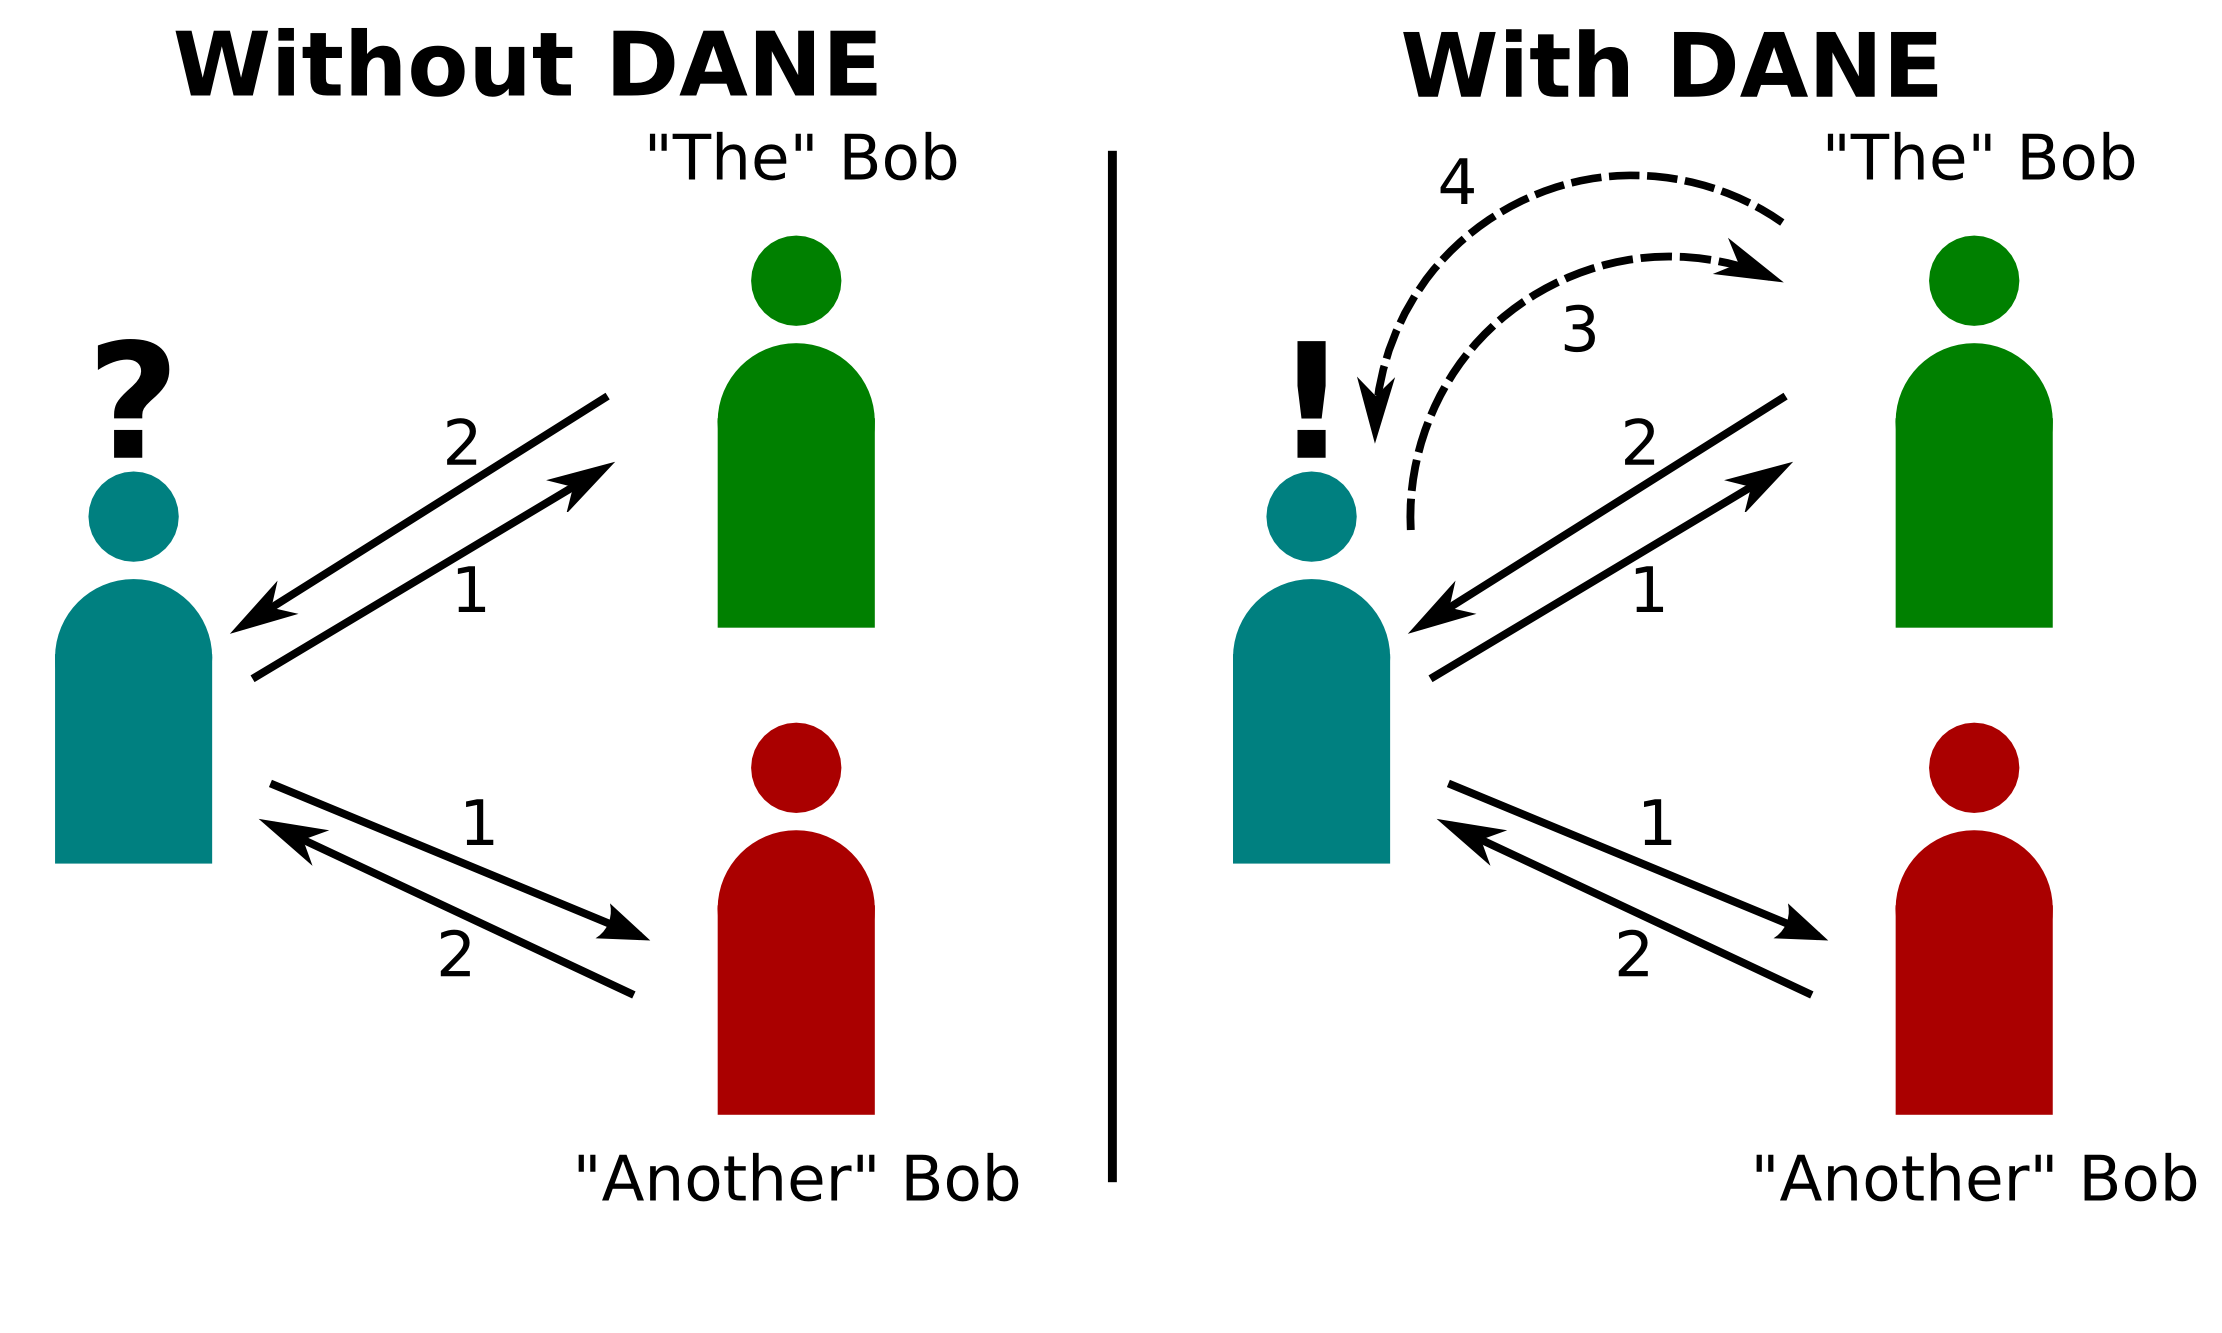
\includegraphics[scale=1]{Figures/daneWithAndWithoutDane.png}
\end{center}
\caption{Without DANE the connecting client can't be sure without some out-of-band procedure or prior communication who is the real Bob. With DANE "the" Bob can publish a TLSA RR which will determine which TLS server certificate is the real one. (This assumes that both the client and "the" Bob trust the DNSSEC infrastructure).\label{ch3:daneWithAndWithoutDane}}
\end{figure}


Hold on, how does Alice know that she is communicating with "the" Bob she believes it is or is it someone else that is trying to fake the identity of "the" Bob?
To perhaps give a better explanation figure \ref{ch3:daneWithAndWithoutDane} describe this dilemma.

In the initial TLS handshake Alice retrieves a server certificate that she needs to validate with a third party, a CA.
This is a certificate from Bob that is signed by his CA of choice, which basically says that the CA in question has confirmed, in some out-of-band way, that it's the true Bob, Alice is communicating with.

In this scenario, similiar to the scenario with the "hacker" above, there is no way for Bob as server/domain owner to limit which certificates that is allowed to be used for his domain.
A hacker with a certificate for Bob's domain signed by any well-known CA will be able to set up his/her valid TLS server in the name of Bob.
Alice will then never know if it really is "the" Bob she is communicating with next time.

To prevent this Bob can publish TLSA DNS resource records (TLSA RRs)\cite[ch. 2]{rfc:draft-dane} with either the full certificate or a hash value of it.
Alice can when initiating the TLS handshake also ask for the TLSA RRs from Bob.
With DNSSEC in place she can be sure that she recieves the TLSA RR from the true Bob and if the resource records matches the given certificate that was given in the TLS handshake Alice is sure it's to "the" Bob she is opening a secure channel.

Depending on the TLSA RR information and local policies Alice might have to do the the normal certificate chaining to some trusted anchor as well or she will accept a self-signed certificate from Bob.
TLSA resource records is a new DNS record type that is still not approved as a standard so it might change in the future before being approved.

% TODO: Give more in depth presentation about certificate here?
% TODO: Mention anywhere what root certificates are and how they're used?
% TODO: What is well-known CAs?

% Removed by Christoffer, 2012-04-19: As the Internet-Draft specifies the first octet in the TLSA RR is allocated for "certificate usage", the parts concerning TLS only allocates five out of these 256 possible values so future standards can use the same resource record type and only allocating one of the free "certificate usage" fields.
% Removed by Christoffer, 2012-04-19: This means that if a new standard is created that doesn't make use of TLS but needs certificate in some other way it might make sense to allocate a "certificate usage" number within the TLS RR instead of creating whole new resource record type.

% TODO: ADD: With DANE the CA system remains the same with two big differences.
% (1) Without DANE all CAs are as weak as the weakest CA. Every CA needs to make sure to keep their private keys/certificate safe.
% If anyone of them brakes, all CAs lose trust. With DANE only domains originally signed by themselves is in danger for false certificate so if a warning goes out fast when the break-in is noticed...zone administrators in danger can revoke their certificates asap and publish a new in the DNS system. (Though even the false certificate from the hackers may not be of any help)...though better be safe than sorry if any private key from a CA is lost.
% (2) With DANE it will still be possible to hack a CA and create false certificate for any domain but with DANE the additional check can be made through the DNS system and the zone owner/administrator has the last say when it comes to which certificates that are the true ones.

\section{How DANE can be implemented in Shibboleth}
Shibboleth is not a single computer program, it's more of a software package consisting of an identity provider written in java and a service provider written in C++ as the main parts.
As dependency for the identity provider and service provider software, Opensaml exist both in Java and C++.
Other projects are a centralized discovery service, embedded discovery service and  metadata aggregator among others.
Even if Shibboleth can be viewed as a software package, all parts can and usually are installed seperately on different machines.

DNS-Based Authentication of Named Entities (DANE) is still a draft for TLS and S/MIME communication and the RFC available is only an informational RFC focusing mainly on TLS use cases.
The main concept is that with DNSSEC in place it's possible to use the DNS system as a trusted source for retrieval of some extra information that confirms what earlier was made in some other out-of-band way.
As an example it's possible to trust a TLS certificate retrieved when establishing that connection because it's possible to retrieve extra information through the DNS system that proves it's the right certificate in use.

Focus has been put on the identity provider part in Shibboleth.
It has good documentation on how to extend it. 
Make note that the identity provider software is currently at version 2.3.6 and a new major version is on the way as 3.0.0.
The identity provider software has both an API and different extension points.


%Migh be implemented as a filter in shibboleth IdP
%There are several "layers" in the Shibboleth software
%Shibboleth uses OpenSAML and OpenSAML uses OpenSSL(confirm this later on.)

%DNS (Domain Name System) is the Internets domain name system, a hierarchic and distributed database that makes it possible to quickly find information about which IP-address (and other information) that is connected to a domain name. \cite[p.~64]{book:guide_dns}

%DNSSEC (Domain Name Security Extensions) is a securitylayer added to DNS to secure system against assults like cachingpoisning through signing DNS-data digitaly.\cite[p.~64]{book:guide_dns}

%\section{Theories}

%How do they work together?

%\section{Tools}

%Software? Shibboleth?


%THEORY 
%Background, 
%theories, 
%tools, 
%and anything else that can be used in your work.
%These are largely determined by your purpose and delimitations. This puts your investigation
%in its scientific context.


\makechapter{Evaluation}{Evaluation\label{ch4}}
\section{How to improve security for identity federations}
%Security in identity federations involves data integrity, which is said to be true when
%the federations entities can share trusted metadata between each other. 
%The metadata is trusted when the entities in the federation can identify each other with the help of 
%certificates within the metadata file.

%Messages sent between entities depend on the data integrity being held.
Messages sent between entities within the identity federations depends on the data integrity being held.
However, the most difficult part is setting up SAML's first trust relationship between entities, the first exchanging of keys.
The SAML metadata document talks about various mechanisms "to aid in establishing trust in the accuracy and legitimacy of metadata,
including use of XML signatures, SSL/TLS server authentication, and DNS signatures.
Regardless of the mechanism(s) used, relying parties SHOULD have some means by which to establish trust in metadata information
before relying on it" \cite[p.~29]{pdf:oasis-open-metadata}.

With that said, after the first certificate exchange has been made a trust relationship is built and the data integrity is up and running. 
The question is, how can the first certificate exchange be made securely? 
One solution might be a third party, a CA or the use of DNSSEC or maybe both to validates that the certificates is the right ones.
Another one could be to use Pretty Good Privacy (PGP)  \cite{rfc:2440} to sign or encrypt the certificate before transmission.
With this solution, the soon to be certificate receiver first sends a PGP encrypted message containing its contact
information to the certificate sender, that decrypts the message. Finds out the receivers phonenumber and calls him or her
to confirm the message sender and key used in the PGP message.
When it is confirmed that it came from the receiver, the certificate sender sends the certificate to the receiver.

Furthermore, the communication standard described in SAML could be more restricted.
That involves the first certificate exchange just mentioned. 
Another example is the certificate itself, the SAML bindings document says  
that the bindings which use TLS/SSL has to authenticate clients using X.509 certificate \cite[p.~8]{pdf:oasis-open-bindings} and the metadata profile document says that 
"in the case of an X.509 certificate, there are no requirements as to the content of the certificate apart from the requirement 
that it contain the appropriate public key. 
Specifically, the certificate may be expired, not yet valid, carry critical or non-critical extensions or usage flags, and contain 
any subject or issuer. 
The use of the certificate structure is merely a matter of notational convenience to communicate a key and has no semantics in this 
profile apart from that. 
However, it is RECOMMENDED that certificates be unexpired" \cite[p.~11]{pdf:oasis-open-metadata-profile}. 

By changing the SAML documents guidelines in general to be less open for interpretation it could improve the security. 
For example to not recommend that the certificates has not expired, but express that they should or must not be expired. 
Moreover, it is a vulnerability that the metadata file can contain expired certificates.

Without stricter guidelines an online check of the certificate could also be a solution to the expired certificate problem. 
The Online Certificate Status Protocol (OCSP) \cite{rfc:6277} could be used to perform this online check.

\section{How to combine identity federations and DANE}
As stated earlier it's possible to divide federations into two categories, those with a federation provider and those without.
In the analysis that has been done the solution with a federation provider is the most probable and viable setup in the long run, it's basiclly much easier to scale, both technically and non-technically.
It's with this configuration in mind the following evaluation has been made.

%TODO: (1) Kontrollera att det finns information om båda kategorierna av federationer.
%TODO: (2) Kontrollera att analys är gjord och att det verkligen är varianten med en FO som är mest trolig.

With a federation provider publishing all the metadata about all service providers, identity providers and other entities how do the trusting entites rely on the federation provider?
Is it the correct federation provider the trusting entities connect to or is it someone trying to "impersonate" the role of the federation provider as a man-in-the-middle attack.

As of now the trust must be made in some out-of-band way e.g. a simple download of the federation provider's certificate and then confirm it's the correct one via telephone, email communcation between administrators or meet in person.
This is not very practical when the federation grows bigger with tenths or hundreds of service- and identity providers or is it the only way?
\subsection{The publishing problem}
\subsubsection{SAML2 certificate as CERT resource record}
\label{subsec:saml2-certificate-as-tlsa}
The first solution that comes into mind is that it might be possible to publish the federation provider's certificate in the Domain Name System and more specifically as a CERT RR\cite{rfc:4398}.
This would mean that when a requesting entity (service provider, identity provider or any other entity) needs to update the metadata about all other entities it connects to the federation provider and downloads the metadata.
At the same time the requesting entity sends out a DNS lookup (with DNSSEC active) for a corresponding CERT RR.
When both the metadata and the CERT RR is retrieved, a comparison can be made and confirm or dismiss the validity of the metadata.

A problem that still exists with this approach is how will each entity transmit metadata about itself to the federation provider and how will the metadata be validated by the federation provider.
To keep building on the same solution each entity would have to publish respective certificate as a CERT RR themselves in their own domain zone.
They would also need to sign their own metadata which is not the case in current standards. 
Now the initial upload of metadata from an entity to the federation provider could be intitated, perhaps through a web interface, with or without some "Pretty Good Privacy" (PGP) solution e.g. OpenPGP\cite{rfc:2440}.
% TODO: Add use cases from registry->registrar in DNS and how it is used their.
The federation provider than fetches the metadata aswell as the corresponding CERT RR from the entity and if it's the correct signature on it the federation provider can publish it with the metadata from all other entities.
Within one cache interval all entities will now fetch the complete updated metadata from the federation provider.

% TODO: What is a cache interval?
% TODO: What is a domain zone?

New questions arises here, is it practical to store SAML2 certificates in the Domain Name System as a CERT RR?
The second question that comes to mind is more related to DANE.
If CERT RRs is used as stated above it would require DNSSEC otherwise its value would be of no use.
Is it not possible to just use the TLSA RR with TLS certificates as it is and not introduce another layer that CERT RRs would become within the same system (DNS and DNSSEC)?

\subsubsection{Only use TLS (with TLSA RR)}
\label{subsec:only-tlsa-rr-with-tls}
Let's start with the second question and get back to the first one later on.
The solution is already at the point where all entities within a federation needs to sign their own zone with DNSSEC as an underlying infrastructure.
Instead of publishing SAML2 certificates in the Domain Name System it might be possible to just use TLS with TLSA RRs and deem that all the information communicated between any two entities is valid as long as it's over TLS that has been established with TLSA RRs procedures.

This would mean that when a new entity, let's say a service provider, joins a federation the service provider must send its metadata to the federation provider.
As an example the administrator for the service provider might visit a webpage over HTTPS (with validity check for TLSA RR) to initiate the transfer of metadata.
The federation provider than opens a new connection over HTTPS (with validity check for TLSA RR) for the metadata from the service provider.
This request from the frederation provider back to the requesting service provider is to make sure that the metadata that is fetched is from the right service provider. 
When the metadata is recieved the federation provider can publish it with the metadata for all other entities.

% TODO: What is metadata?
% TODO: What is an entity?

\subsubsection{Publishing SAML2 certificate as CERT RR, is it viable?}
\label{subsec:saml2-certs-in-cert-rr}
Earlier in this chapter the question arose if it is practical to store SAML2 certificates in the Domain Name System.
As this is out of scope of this report further investigations has to be done in this area.
For further discussions it's assumed that it's a viable solution to store SAML2 certificates in the Domain Name System as CERT RRs.

\subsubsection{Using the best of two worlds}
It's often the simple solutions that are the best ones but would it be worth it to use TLSA validated connection for the https communication together with the SAML2 certificates in CERT RRs as explained in earlier sections?

To simplify the view an argument could be made that the validity check on the SAML2 certficate downloaded over the HTTPS secure channel and then verified against the CERT RR is just another safety check within the same "layer" as the secure channel was established in.
The reason for this is that the TLS connection is validated first with information from the DNSSEC infrastructure, when requesting the TLSA RR.
The second validation is made depending on the TLSA RR information and local policies, it confirms that the TLS server certificate chain is to be trusted or not.
The third validation would be when the SAML2 certificate is compared against the CERT RR available within the DNSSEC infrastructure.

As noted the first and the third validation are both trusting the DNSSEC infrastructure, and therefore the combination of both using TLS with TLSA and SAML2 certificate with CERT RRs would at first glance not add any extra benefits.
Though under some circumstances someone might be able to hack into a webserver for some entity and change the SAML2 certificate, the third validation check against the CERT RR would in this case fail.
So in the end the question boils down to if the communication is secure to the correct host is this enough to trust everything that the host sends?

\subsection{The matching dilemma}
\label{subsec:matching-dilemma}
The last section was about how to distribute the certificate within the Domain Name System and if it's necessary or not.
The CERT RR is mentioned as a possible solution and there might be several other solutions aswell.
If it's decided upon that a TLSA validated TLS connection is not enough to trust the data that is being sent the SAML2 certificates must be published aswell in the Domain Name System.
With a single or just a few certificates that signs all metadata files for the federation provider it's relatively easy to publish the certificates in the Domain Name System and fetch all of them based on the domain/subdomain.
Though it would put an unwanted limit that the federation provider is only allowed to use a few certificates per DNS zone.
Of course it would work with several hundred certificates but it wouldn't be a very good solution.
This is because each time some entity would check if the certificate is the correct one the requesting entity would have to download all certificates through the Domain Name System and then one by one try to match them against the certificate used in the metadata file.

This means that somekind of general algorithm/solution is required to locate the correct certificate published in the Domain Name System when an entity recieves a signed metadata file.
One way of doing this might be with the "Dynamic Delegation Discovery System (DDDS)"\cite{rfc:3401,rfc:3402,rfc:3403,rfc:3404} and the NAPTR resource record\cite{rfc:3403}.
Exactly how this could be done is out of the scope of this report.

The main issue in this section on how to find the "right" certificate if it's decided upon to publish SAML2 certificates within the Domain Name System was originally formulated by Leif Johansson (SUNET).

\section{How DANE can be implemented in Shibboleth} 
DANE as a technology is on the way to becoming a standard within TLS communication and sooner or later also for S/MIME.
There is not even a draft available for the use together with certificates concerning other usages than those, therefore there is no way to "implement" DANE for Shibboleth (concerning the SAML2 certificates that is).
What has been implemented is more of a proof-of-concept for future reference if/when there is a standard available.

The implementation has been solely done on the Identity provider to keep our focus on one implementation instead of trying to implement it on both the service provider and identity provider software.
Main reason for this has beeen time constrains.

As stated in previous chapter the software for the identity provider part is written in Java.
It has several API access points aswell as several extension points where the functionality of different parts can be extended.
The implementation finally made was a "TrustEngine"-extension.
A TrustEngine is a part of Shibboleth that processes either metadata or other messages to validate it or dismiss the message.
A example TrustEngine is the "ExplicitKeySignatureTrustEngine" that takes one or more certificates and some signed metadata and confirms that the signature is the right one. 

% TODO: More research into this? Perhaps we will give an answer to this that is enough.

%\section{Temporary section}
%EVALUATION This is where you put the spotlight on your solution's strengths and
%weaknesses. An evaluation must be made of the methods/theory applied and the validity
%and reliability of the data. You should describe the most interesting results of your work in a
%results section. Remember that less important but complementary results can to advantage
%be placed in appendices. A rule of thumb is that all results that you use in your analysis and
%in your conclusions should be reported in the Evaluation chapter and the rest reported in
%appendices.



\makechapter{Discussion}{Discussion\label{ch5}}
\section{Our conclussions}
\subsection{Identity federations with SAML2 and DANE}
We started out with the task to identify where we could improve security within idenitity federations.
We were tasked specifically to look at the data integrity part of SAML2, how X.509 certificates are used and how it would be possible to improve security with the help of DNS-Based Authentication of Named Entities.

Our conclussions are that as soon as the initial configuration for each entity in an identity federation is done and all entities are up and running, data integrity is as secure as the public/private key cryptography scheme.
The hard part is still the initial setup on how to decide who to trust when you don't trust anyone online.
Procedures for this is as of today not specified in any detail, it's up to each federation to decide on their own.
Common practice is as said in earlier chapters to share key or certificate information in some out-of-band way e.g. meeting in person or call each other.
We believe that it's this initial sharing of information that would benefit the most if it could be done solely over the internet and it's possible if we put trust in the DNSSEC infrastructure.

DANE is one way to go and is a valid solution for identity federations.
Exactly how to store SAML2 certificates and how to retrieve the correct certificate for each validation of metadata is still an open question we haven't been able to reach that far.
We have listed some solutions such as using CERT resource records and perhaps locating the correct certificate with "Dynamic Delegation Discovery System (DDDS)" procedures.

Our belief is that within future SAML specifications and/or when establishing new federations, more strict rules concerning metadata must be agreed upon to secure the data integrity of the metadata.
Future agreements should include requirements that TLS with TLSA validation is used when sharing metadata.
Another requirement should be to publish the certificates within the DNS/DNSSEC infrastructure.
This is to make sure that both the channel that the communication is taking part over is secure aswell as the data stored on the webserver accessed is the proper one e.g. if downloading a certificate over a HTTPS connection.
DANE may be used, instead of, or as an addition to current procedures.


\subsection{Proof of concept}
TODO - Implementation

%DANE
%Säkra både TLS och certifikat eftersom webbserver kan hackas men inte så troligt att även zonen blir hackad eftersom det är vanligt att placera en master server bakom många slav-servrar som är blåttade mot omvärlden.


%Connect back to the topic under "Chapter 1: Purpose". Do we reach our purpose?
% TODO: Make comments about that if we can secure the transmission of Metadata between all entities (FOs, IdPs, AAs, SPs and Discos) we can deem that the data integrity of all messages transmitted between them(the entities) is not lost or tampered with. As long as all entities do a proper check for each SAML2 message.

\section{How to continue with further research}
\subsection{Communication with a federation provider}
The communication between the federation provider and the other entities such as identity providers and service providers has no standardized way in how it should work.
How does the federation provider know that it really is the right identity provider it's talking with, without any prior communication?
Should the federation provider be the one that initiate connection to the other entities or vice versa?
Last, but no least, how should this be solved technically to minimize the manual labour and automate as much as possible?

\subsection{SAML2 certificates in CERT resource records}
In section \ref{subsec:saml2-certs-in-cert-rr} it's mentioned that SAML2 certificates could be stored in CERT RRs.
Further research need to be done to establish exactly how this could be accomplished.
With CERT RR it's possible to store the certificate in it's full format, only a hash of it or just a url to the location where it's stored\cite[ch. 2.1]{rfc:4398}.
What would be suitable for SAML2 certificates and is this really a viable solution for the identity federation scheme?

\subsection{How to use NAPTR RRs to find the correct SAML2 certificate}
In section \ref{subsec:matching-dilemma} "Dynamic Delegation Discovery System (DDDS)"\cite{rfc:3401,rfc:3402,rfc:3403,rfc:3404} and the NAPTR resource record\cite{rfc:3403} is mentioned as a possible solution to the "matching problem".
How does an entitiy that has recieved a signed metadata file locate the correct certificate within the Domain Name System?

%\section{Temporary section }
%DISCUSSION Your conclusions, where you link your findings to your theories and purpose,
%will discuss whether you achieved your purpose and what opportunities exist for further
%development. An analysis and interpretation of your results may often correspond to the
%frame of reference and the theoretical models you have used. Using models, checklists etc,
%you broke down your task into manageable questions. Now you reverse your approach and
%use them to build general conclusions and recommendations that correspond to your
%purpose and your client's decision situation.



%%==================================================================
%% Include any appendices here.
%%==================================================================
\appendix % This command initializes the appendix part, Don't change!

%% Include appendix A, add more if needed
\makeappendix{Appendix A}{Titel p� appendix A\label{appA}}
Appendix A (appendixA.tex)

TODO Here is a "nocite" latex command that needs to be removed when final printing is to be done. The nocite command below include all references in our bibliography but it's not certain if we have used them all.
\nocite{*}


%%==================================================================
%% Include bibliography references here
%% Replace the "thesisreferences" with your
%% own reference database
%%==================================================================
\bibliographystyle{ieeetr}

\fancyhead[LO]{}%
\fancyhead[RE]{}%
\fancyhead[LE]{\thepage}%
\fancyhead[RO]{\thepage}
\bibliography{thesisreferences}

\end{document}
